\chapter{Blok p II: Oksigen, Halogen, dan Gas Mulia}\label{ch:b1:p-block-16-18}

Asam sulfat dibuat dalam tonase yang lebih besar daripada bahan kimia lain
mana pun: asam itu melarutkan batuan fosfat untuk pupuk, melindi bijih
tembaga dan uranium, memurnikan minyak bumi, dan mengisi aki mobil, dan
selama satu abad produksi asam sulfat menjadi ukuran kasar industri
sebuah negara. Sebagian besar belerangnya kini berasal dari pembersihan
gas alam dan minyak bumi; sebagian masih dipikul dengan tangan keluar dari
kawah gunung api. Belerang terletak dalam \omterm{def:b1:periodicity:table}{golongan} 16 di bawah oksigen;
\omterm{def:b1:p-block-16-18:halogen}{halogen} \omterm{def:b1:periodicity:table}{golongan} 17 dan gas mulia \omterm{def:b1:periodicity:table}{golongan} 18 melengkapi \omterm{def:b1:periodicity:table}{blok} p. Bab ini
mengikuti oksigen dan belerang dari unsurnya sampai asamnya, mengurutkan
\omterm{def:b1:p-block-16-18:halogen}{halogen} sebagai \omterm{def:b1:nernst:couple}{oksidator} dengan \omterm{def:b1:nernst:electrode-potential}{potensial standarnya}, dan diakhiri
dengan senyawa-senyawa yang ternyata memang dibentuk oleh gas mulia yang
konon inert.

\begin{recall}
\omterm{def:b1:lewis-resonance-vsepr:lewis}{Struktur Lewis}, oktet yang diperluas, dan bentuk-bentuk VSEPR (\cref{ch:b1:lewis-resonance-vsepr});
\omterm{def:b1:nernst:electrode-potential}{potensial standar} (\cref{ch:b1:nernst}); \omterm{def:b1:e-ph-diagrams:disproportionation}{disproporsionasi} klorin dan
\omterm{def:b1:e-ph-diagrams:e-ph-diagram}{diagram potensial--pH} klorin (\cref{ch:b1:e-ph-diagrams}); katalisis
(\cref{ch:b1:elementary-steps}). Jilid sekolah (kelas 10) telah
mengelompokkan \omterm{def:b1:p-block-16-18:halogen}{halogen} dan gas mulia sebagai keluarga.
\end{recall}

\begin{omfigure}
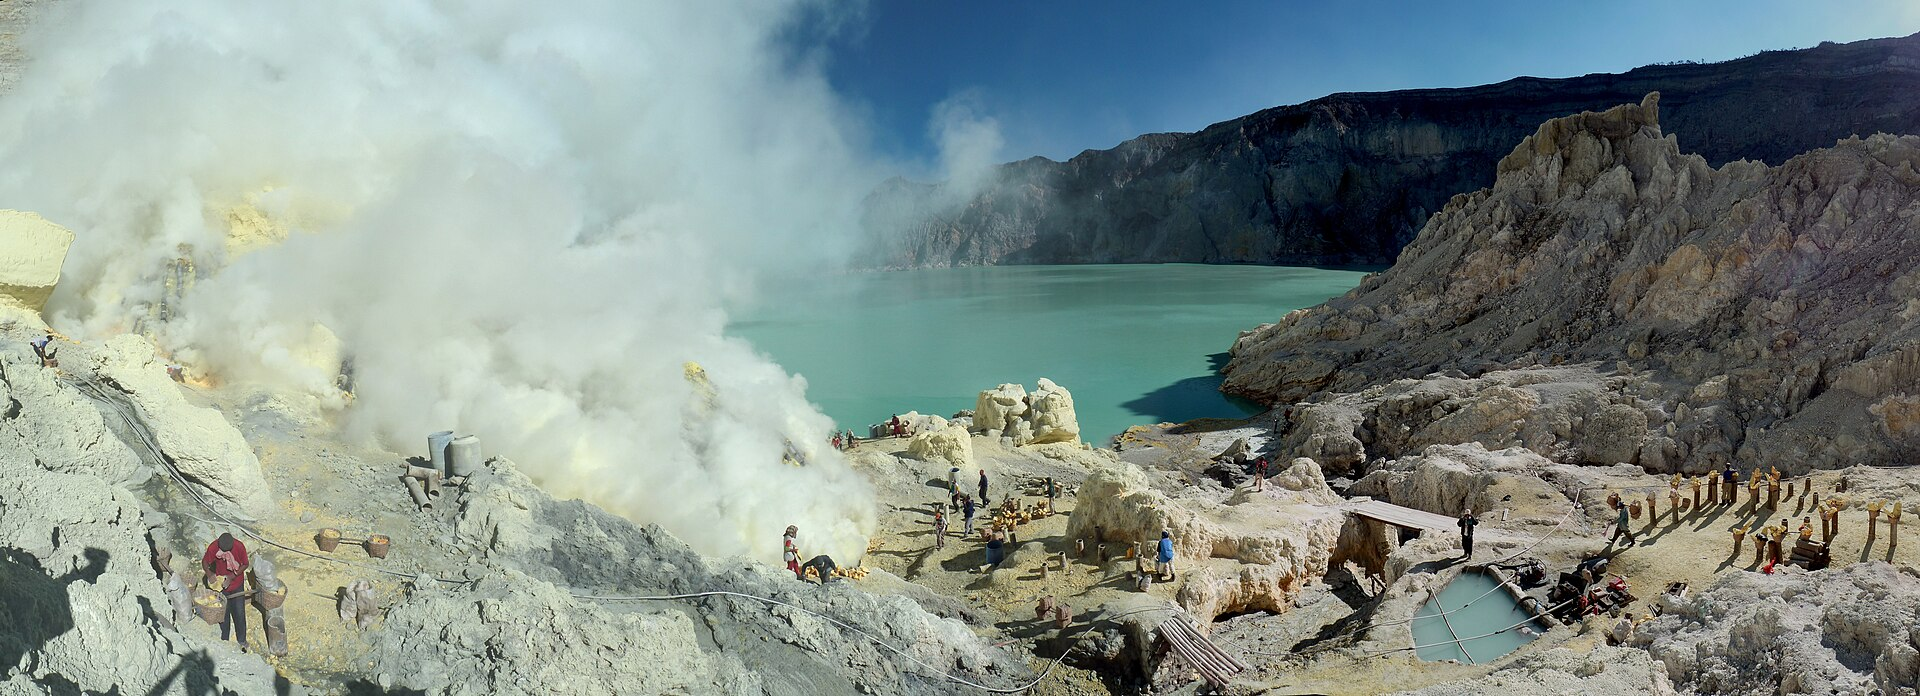
\includegraphics[width=0.78\linewidth]{images/book2/kawah-ijen.jpg}

{\small Penambangan belerang di kawah Gunung Ijen (Kawah Ijen), Indonesia:
gas-gas vulkanik mengembunkan belerang kuning di sekitar pipa-pipa, dan
para penambang memikulnya keluar dalam keranjang (foto Sémhur, CC BY-SA
4.0, Wikimedia Commons).}
\end{omfigure}

\section{Oksigen, ozon, dan peroksida}

\begin{definition}[Kalkogen]\label{def:b1:p-block-16-18:chalcogen}
\emph{Kalkogen}\index{kalkogen} adalah unsur-unsur \omterm{def:b1:periodicity:table}{golongan} 16 (O, S, Se,
Te, Po), dengan enam \omterm{def:b1:quantum-numbers:configuration}{elektron valensi} \textit{ns}$^2$\textit{np}$^4$.
Unsur-unsur itu membentuk senyawa dengan \omterm{def:b1:nernst:oxidation-number}{bilangan oksidasi} dari $-$II
(oksida, sulfida) sampai $+$VI (sulfat); \omterm{def:b1:nernst:oxidation-number}{bilangan oksidasi} yang tinggi
hanya dicapai belerang dan unsur di bawahnya.
\end{definition}

Oksigen terdapat sebagai dioksigen \ce{O2} dan sebagai ozon \ce{O3},
molekul bengkok dengan dua \omterm{def:b1:lewis-resonance-vsepr:resonance}{struktur resonansi}
(\cref{ch:b1:lewis-resonance-vsepr}). Ozon adalah \omterm{def:b1:nernst:couple}{oksidator} yang lebih
kuat daripada dioksigen: $E^\circ(\ce{O3}/\ce{O2}) = 2.07$~V
dibandingkan dengan 1.23~V untuk \ce{O2}/\ce{H2O}. Di atmosfer atas, ozon
menyerap sinar ultraviolet; di dekat permukaan tanah, ozon adalah
pencemar. Hidrogen peroksida, dengan ikatan \ce{O-O} dan oksigen pada
$-$I, adalah \omterm{def:b1:nernst:couple}{oksidator} sekaligus \omterm{def:b1:nernst:couple}{reduktor} dan mengalami \omterm{def:b1:e-ph-diagrams:disproportionation}{disproporsionasi}
secara lambat (\cref{exo:b1:nernst:12}).
% ledger: dfg:O3_g (E0 computed in figdata/bachelor-1/standard-potentials.py)

\begin{example}[Bilangan oksidasi oksigen]
Oksigen, yang \omterm{def:b1:periodicity:electronegativity}{keelektronegatifannya} hanya kalah dari fluorin, berada pada
$-$II dalam hampir semua senyawanya: air, oksida, hidroksida, sulfat.
Pengecualiannya mengikuti aturan bahwa elektron yang dipakai bersama
diberikan kepada pasangan yang lebih elektronegatif dan dibagi sama rata
antara atom-atom yang identik. Dalam hidrogen peroksida \ce{H2O2},
H--O--O--H, setiap oksigen mengambil elektron ikatan \ce{O-H}-nya tetapi
membagi pasangan \ce{O-O}: $-$I. Dalam kalium superoksida \ce{KO2}, ion
\ce{O2-} membawa satu muatan untuk dua atom:
$-\frac12$ rata-rata. Dalam oksigen difluorida \ce{OF2}, fluorin
memenangkan kedua ikatan dan oksigen berada pada $+$II. Dalam \ce{O2} dan
\ce{O3}, oksigen berada pada 0. Hanya keadaan $-$II yang stabil terhadap
air; peroksida dan superoksida adalah \omterm{def:b1:nernst:couple}{oksidator}, dan \ce{OF2} adalah zat
pemfluorinasi.
\end{example}

\section{Belerang dan asam sulfat}

Belerang, tidak seperti oksigen, membentuk cincin dan rantai ikatan
tunggal \ce{S-S}: belerang biasa tersusun atas cincin \ce{S8}. Belerang
terbakar menjadi belerang dioksida, molekul bengkok (sudut O--S--O
\ang{119.5}), yang dapat dioksidasi lebih lanjut menjadi belerang
trioksida, yang berbentuk segitiga datar. Keduanya adalah \omterm{def:b1:s-block:oxide-character}{oksida asam}:
\ce{SO2} menghasilkan asam sulfit ($\mathrm{p}K_a$ 1.77 dan 7.22), \ce{SO3}
menghasilkan asam sulfat.
% ledger: geo:SO2.aOSO, dfg:SO2_g, dfg:SO3_g

\begin{proposition}[Tahap-tahap proses kontak]\label{prop:b1:p-block-16-18:contact-steps}
Asam sulfat dibuat dari belerang dalam empat tahap:
(1) \ce{S + O2 -> SO2}; (2) \ce{2SO2 + O2 <=> 2SO3}, di atas \omterm{def:b1:elementary-steps:catalyst}{katalis}
vanadium(V) oksida; (3) \ce{SO3 + H2SO4 -> H2S2O7} (oleum), dengan
trioksida itu diserap ke dalam asam pekat; (4) \ce{H2S2O7 + H2O -> 2H2SO4}.
Secara keseluruhan, \ce{2S + 3O2 + 2H2O -> 2H2SO4}.
\end{proposition}

\begin{proof}
Setiap tahap sudah setara; dengan menjumlahkan $2\times(1)$, (2), $2\times(3)$, dan
$2\times(4)$, \ce{SO2}, \ce{SO3}, dan \ce{H2S2O7} saling meniadakan, dan
kedua \ce{H2SO4} yang terpakai pada tahap 3 terbentuk kembali pada tahap
4, sehingga tersisa \ce{2S + 3O2 + 2H2O -> 2H2SO4}. Tahap 2 sangat disukai
secara termodinamika pada suhu kamar ($K = 10^{24.8}$ pada
\qty{25}{\celsius}, dari energi Gibbs pembentukan), tetapi sangat lambat:
\omterm{def:b1:elementary-steps:catalyst}{katalisnya}, yang hanya aktif dalam keadaan panas, itulah yang membuatnya
berjalan, dan kompromi antara laju dan konversi dipelajari dalam jilid
Tahun~2. \ce{SO3} tidak diserap langsung ke dalam air, karena reaksinya
dengan uap air membentuk kabut halus tetesan asam yang lolos melewati
penyerap.
\end{proof}
% ledger: dfg:SO2_g, dfg:SO3_g

\begin{omfigure}
\begin{tikzpicture}[font=\small, >={Stealth}, box/.style={draw, rounded corners, fill=omDef!8, align=center, minimum height=1.0cm}]
  \node[box] (b) at (0,0) {tungku belerang\\\ce{S + O2 -> SO2}};
  \node[box] (c) at (4.4,0) {konverter, \ce{V2O5}\\lapisan katalis};
  \node[box] (a) at (8.8,0) {menara absorpsi\\\ce{SO3} ke dalam \ce{H2SO4}};
  \node[box] (d) at (8.8,-2.2) {pengenceran\\\ce{H2S2O7 + H2O}};
  \draw[<-, thick] (b.west) -- ++(-0.8,0) node[left, align=right] {udara,\\S};
  \draw[->, thick] (b) -- node[above] {\ce{SO2}} (c);
  \draw[->, thick] (c) -- node[above] {\ce{SO3}} (a);
  \draw[->, thick] (a) -- node[right] {oleum} (d);
  \draw[->, thick] (d.west) -- ++(-1.2,0) node[left] {\ce{H2SO4}};
  \draw[->, thick] (d.east) -- ++(0.6,0) |- node[pos=0.25, right, align=left] {sebagian\\dikembalikan} (a.east);
\end{tikzpicture}

{\small Proses kontak: pembakaran belerang, oksidasi katalitik \ce{SO2},
absorpsi \ce{SO3} dalam asam sulfat pekat, dan pengenceran oleum.
Sebagian asamnya dikembalikan ke penyerap.}
\end{omfigure}

\begin{proposition}[Kekuatan asam sulfat]\label{prop:b1:p-block-16-18:sulfuric-strength}
Dalam air, keasaman pertama asam sulfat kuat (sempurna), keasaman
keduanya lemah: $\mathrm{p}K_a(\ce{HSO4-}/\ce{SO4^2-}) = 1.99$. Karena itu,
larutan \qty{0.010}{mol/L} tidak berada pada pH 1.70 (dua proton) maupun
pada 2.00 (satu proton), tetapi di antara keduanya.
\end{proposition}

\begin{proof}
\ce{H2SO4}, dengan dua oksigen tanpa hidrogen pada belerang, adalah \omterm{def:b1:p-block-13-15:oxoacid}{asam
okso} yang lebih kuat daripada \ce{H3O+}: asam itu diratakan
(\cref{ch:b1:predominant-reaction}). \ce{HSO4-}, yang sudah bermuatan
negatif, lebih kuat menahan protonnya: $\mathrm{p}K_a$-nya, yang dihitung
dari energi Gibbs pembentukan, adalah 1.99. Pada $C = 0.010$:
$[\ce{H3O+}] = C + x$, $[\ce{HSO4-}] = C - x$, $[\ce{SO4^2-}] = x$, dengan
$x(C + x)/(C - x) = 10^{-1.99}$; dengan menyelesaikannya, $x = \qty{4.2e-3}{mol/L}$ dan
$\mathrm{pH} = -\log(0.0142) = 1.85$.
\end{proof}
% ledger: dfg:HSO4-_ao, dfg:SO42-_ao

Asam sulfat pekat juga merupakan zat pendehidrasi yang kuat (asam itu
mengarangkan gula dengan mengambil unsur-unsur air darinya) dan, dalam
keadaan panas, sebuah \omterm{def:b1:nernst:couple}{oksidator}. Pengencerannya melepaskan banyak kalor:
asam selalu dituangkan ke dalam air, tidak pernah sebaliknya. Sebagian
besar belerang dunia, sekitar 84 juta ton pada tahun 2025, diperoleh
kembali dari hidrogen sulfida dalam gas alam dan aliran kilang, dan
sebagian besar berakhir sebagai asam sulfat.
% ledger: usgs:S-world-2025

\begin{method}[Neraca massa dalam proses kontak]\label{met:b1:p-block-16-18:contact-balance}
\begin{enumerate}
  \item Gunakan persamaan keseluruhan: satu \ce{H2SO4} per atom S.
  \item Koreksilah untuk konversi tahap 2 (fraksi \ce{SO2} yang
        teroksidasi) dan untuk kehilangan pada absorpsi.
  \item Untuk udara: hitunglah \ce{O2} yang diperlukan (tiga per dua per
        S) dan bagilah dengan fraksinya dalam udara.
\end{enumerate}
\end{method}

\begin{example}[Pabrik yang membakar seribu ton belerang sehari]
Sebuah pabrik membakar \qty{1000}{t} belerang sehari, mengonversi
\qty{99.0}{\percent} \ce{SO2}, dan menyerap \qty{99.9}{\percent} \ce{SO3}.
Maka
$n(\ce{S}) = \num{1000e6}/32.1 = \qty{3.12e7}{mol}$ dan
$n(\ce{H2SO4}) = \num{3.12e7} \times 0.990 \times 0.999
= \qty{3.08e7}{mol}$, yaitu $\num{3.08e7} \times \qty{98.1}{g}
= \qty{3020}{t}$ asam sehari. Sisa \qty{1.0}{\percent} yang tidak
terkonversi keluar sebagai \ce{SO2}: \qty{3.1e5}{mol}, atau \qty{20}{t}
sehari, yang harus dihilangkan dari gas buang. Dioksigen yang diperlukan
adalah $1.5 \times \num{3.12e7} =
\qty{4.67e7}{mol}$; udara, dengan \qty{21}{\percent} \ce{O2}, adalah
\qty{2.23e8}{mol}, atau $V = nRT/p = \qty{5.5e6}{m^3}$ sehari pada
\qty{25}{\celsius} dan \qty{1}{bar}, sebelum kelebihan udara yang
sebenarnya dihembuskan oleh pabrik.
\end{example}
% ledger: air:O2

\section{Halogen}

\begin{definition}[Halogen]\label{def:b1:p-block-16-18:halogen}
\emph{Halogen}\index{halogen} adalah unsur-unsur \omterm{def:b1:periodicity:table}{golongan} 17 (F, Cl, Br,
I, At), dengan tujuh \omterm{def:b1:quantum-numbers:configuration}{elektron valensi} \textit{ns}$^2$\textit{np}$^5$.
Unsur-unsur itu terdapat sebagai molekul diatomik \ce{X2} dan membentuk
ion halida \ce{X-}.
\end{definition}

\begin{omfigure}
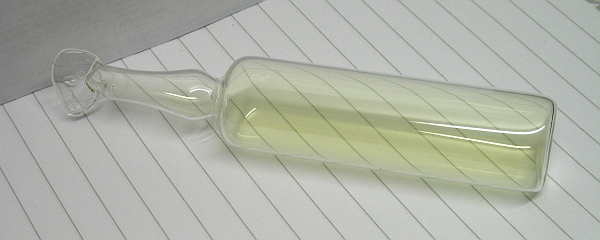
\includegraphics[height=2.9cm]{images/book2/chlorine.jpg}\hspace{0.5em}%
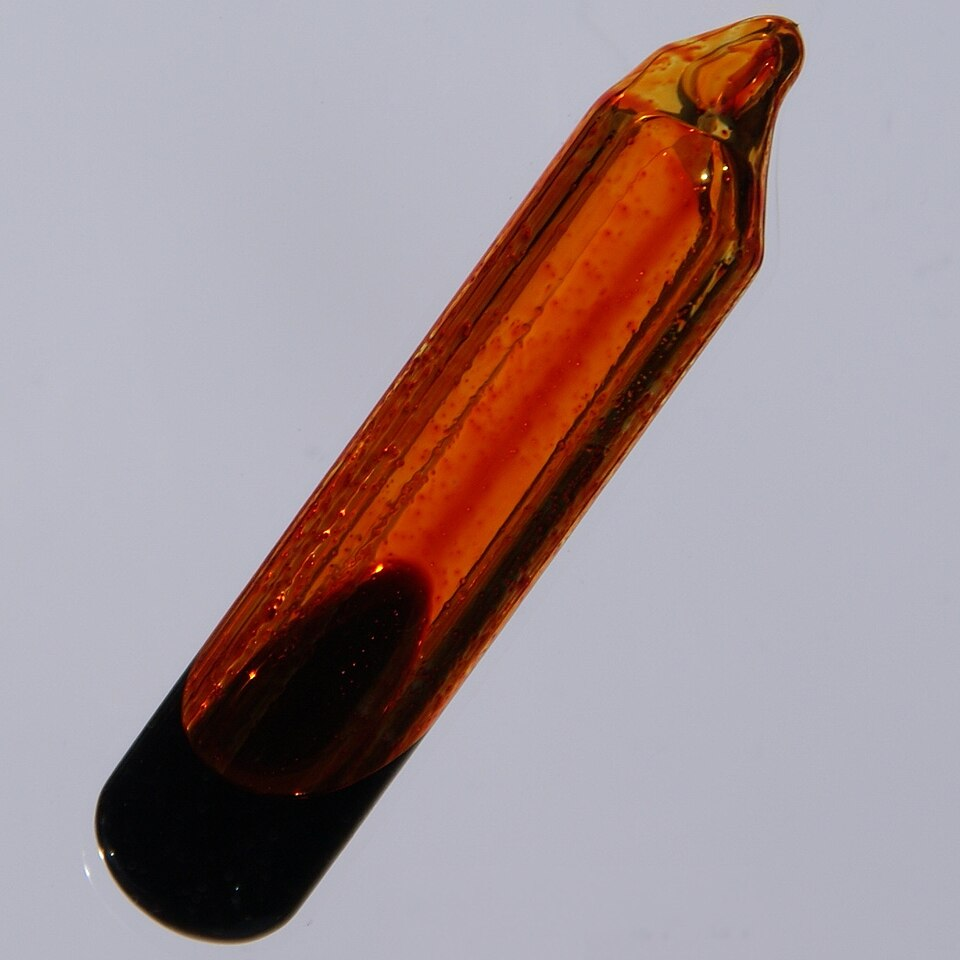
\includegraphics[height=2.9cm]{images/book2/bromine.jpg}\hspace{0.5em}%
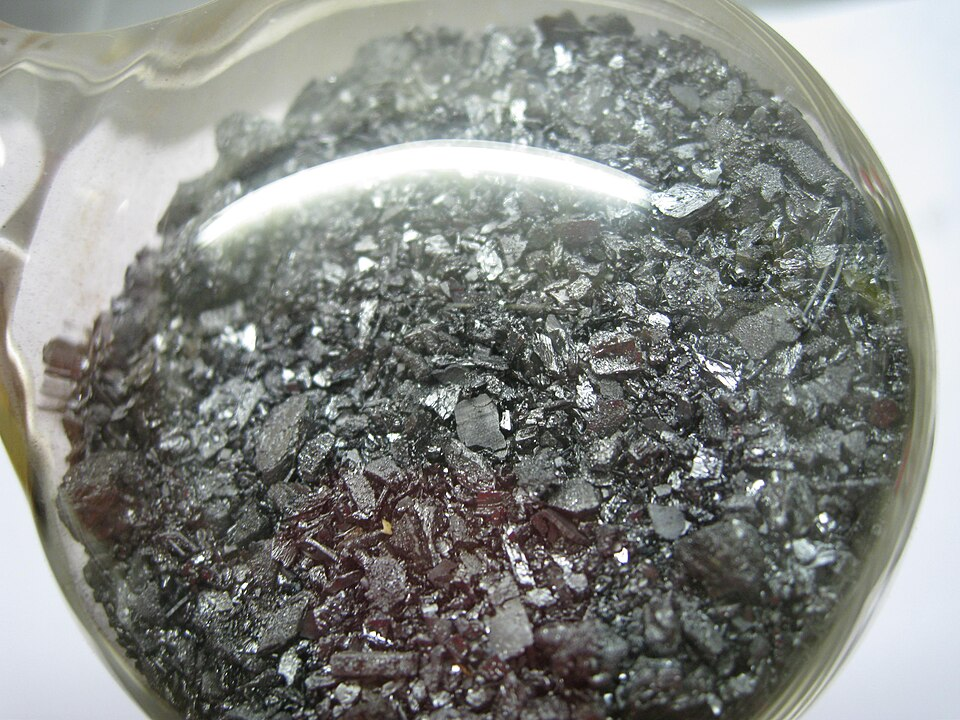
\includegraphics[height=2.9cm]{images/book2/iodine.jpg}

{\small Klorin, gas berwarna kuning kehijauan pucat (W. Oelen, CC BY-SA
3.0); brom, cairan merah tua dengan uap berwarna jingga (Jurii, CC BY
3.0); iodin, \omterm{def:b1:crystals-metals:crystal}{kristal} abu-abu kehitaman dengan kilap logam (Dnn87, CC BY
3.0). Klorin dan brom disegel dalam ampul kaca. Semuanya dari Wikimedia
Commons.}
\end{omfigure}

\begin{proposition}[Daya oksidasi halogen]\label{prop:b1:p-block-16-18:halogen-oxidising-order}
\omterm{def:b1:p-block-16-18:halogen}{Halogen} adalah \omterm{def:b1:nernst:couple}{oksidator} yang kekuatannya menurun ke bawah \omterm{def:b1:periodicity:table}{golongan}:
$E^\circ(\ce{F2}/\ce{F-}) = 2.89$~V, \ce{Cl2}/\ce{Cl-} 1.36~V,
\ce{Br2}/\ce{Br-} 1.08~V, \ce{I2}/\ce{I-} 0.53~V. Setiap \omterm{def:b1:p-block-16-18:halogen}{halogen}
mengoksidasi ion-ion halida di bawahnya dalam \omterm{def:b1:periodicity:table}{golongan} itu.
\end{proposition}

\begin{proof}
Nilai-nilai itu berasal dari energi Gibbs pembentukan ion-ion halida
(\cref{ch:b1:nernst}). Menurut aturan gamma, \ce{X2} mengoksidasi \ce{Y-}
jika pasangan \ce{X2}/\ce{X-} terletak di atas \ce{Y2}/\ce{Y-}: misalnya
\ce{Cl2 + 2Br- -> 2Cl- + Br2}, $\log K = 2(1.36 - 1.08)/0.059 = 9.5$.
Ke bawah \omterm{def:b1:periodicity:table}{golongan}, atom-atomnya membesar, afinitasnya terhadap elektron
tambahan dan hidrasi ion-ion halida yang lebih kecil menurun, demikian
pula potensialnya.
\end{proof}
% ledger: dfg:F-_ao, dfg:Cl-_ao, dfg:Br-_ao, dfg:I-_ao

\begin{omfigure}
\begin{tikzpicture}
\begin{axis}[
  ybar, width=0.62\linewidth, height=5.0cm, ymin=0, ymax=3.3,
  symbolic x coords={F,Cl,Br,I}, xtick=data,
  xticklabels={\ce{F2}/\ce{F-}, \ce{Cl2}/\ce{Cl-}, \ce{Br2}/\ce{Br-}, \ce{I2}/\ce{I-}},
  ylabel={$E^\circ$ (V)}, bar width=16pt, nodes near coords,
  every node near coord/.append style={font=\scriptsize},
  tick label style={font=\small}, label style={font=\small}, enlarge x limits=0.2]
\addplot[fill=omThm!40, draw=omThm] coordinates {(F,2.89) (Cl,1.36) (Br,1.08) (I,0.53)};
\end{axis}
\end{tikzpicture}

{\small \omterm{def:b1:nernst:electrode-potential}{Potensial standar} pasangan halogen--halida pada
\qty{25}{\celsius}, yang dihitung dari energi Gibbs yang ditabelkan: daya
oksidasi menurun secara teratur ke bawah \omterm{def:b1:periodicity:table}{golongan}.}
\end{omfigure}

Hidrogen halida semuanya bersifat asam dalam air, tetapi \ce{HF} lemah
($\mathrm{p}K_a$ 3.16) sedangkan \ce{HCl}, \ce{HBr}, dan \ce{HI} kuat:
ikatan \ce{H-F} sangat kuat dan ion fluorida yang kecil terikat dalam
\omterm{def:b1:intermolecular-forces-solvents:hbond}{ikatan hidrogen} yang kuat. Fluorin adalah unsur yang paling
elektronegatif dan \omterm{def:b1:nernst:couple}{oksidator} terkuat dalam tabel itu; fluorin hanya
dapat diperoleh melalui elektrolisis. Asam-asam okso klorin --- asam
hipoklorit \ce{HClO}, asam klorat \ce{HClO3}, asam perklorat \ce{HClO4}
--- makin kuat seiring bertambahnya oksigen tanpa hidrogen, seperti pada
semua \omterm{def:b1:p-block-13-15:oxoacid}{asam okso} (\cref{def:b1:p-block-13-15:oxoacid}); hubungannya dengan
klorida dan klorin telah dipetakan dalam
\cref{ch:b1:e-ph-diagrams}.
% ledger: dfg:HF_ao, dfg:F-_ao

\begin{omfigure}
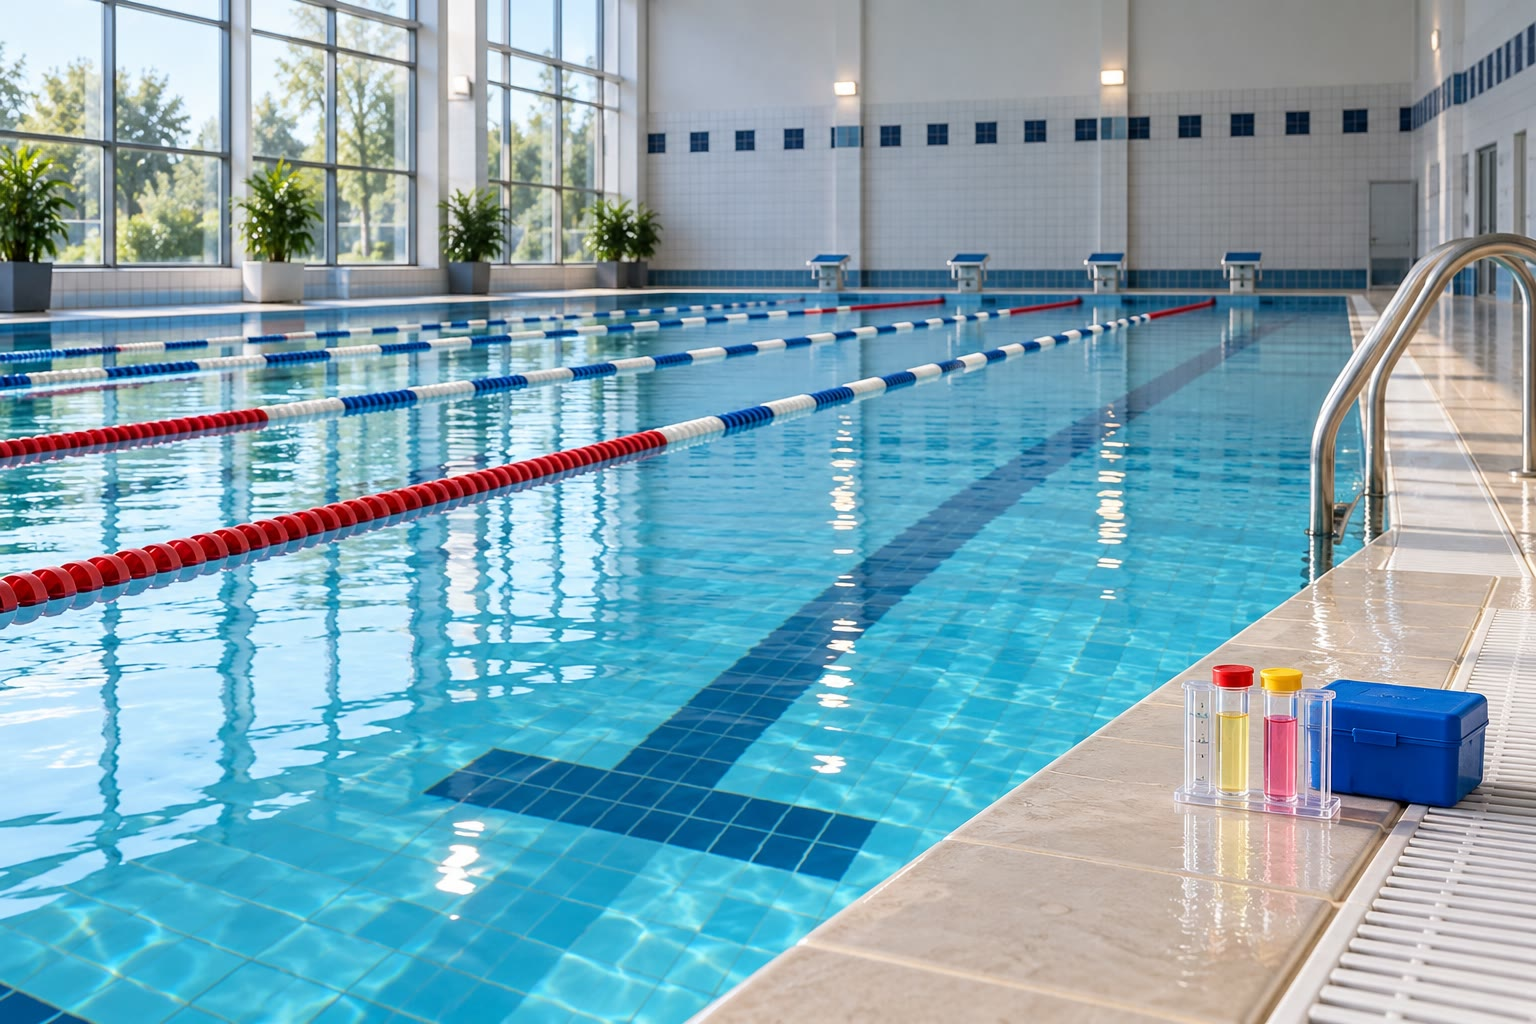
\includegraphics[width=0.55\linewidth]{images/book2/ai/b1-28-swimming-pool.jpg}

{\small Kolam renang umum beserta perangkat uji airnya: klorin yang
terlarut sebagai asam hipoklorit diperiksa beberapa kali sehari.}
\end{omfigure}

\begin{definition}[Senyawa antarhalogen]\label{def:b1:p-block-16-18:interhalogen}
\emph{Senyawa antarhalogen}\index{senyawa antarhalogen} adalah senyawa
dua \omterm{def:b1:p-block-16-18:halogen}{halogen} yang berbeda: \ce{ICl}, \ce{BrF3}, \ce{ClF3}, \ce{IF7}.
\omterm{def:b1:p-block-16-18:halogen}{Halogen} yang lebih besar dan kurang elektronegatif menjadi \omterm{def:b1:complexation:complex}{atom pusat},
dengan oktet yang diperluas pada \ce{ClF3} dan senyawa di atasnya.
\end{definition}

\begin{inthelab}[Menangani halogen]
Klorin beracun dan hanya dibuat dalam jumlah kecil di dalam lemari asam;
brom membakar kulit dan uapnya menyerang paru-paru, dan brom dipakai
dalam keadaan encer, di dalam lemari asam, dengan sarung tangan dan
kacamata pelindung, serta larutan natrium tiosulfat yang siap untuk
merusak tumpahan
(\ce{4Br2 + S2O3^2- + 5H2O -> 8Br- + 2SO4^2- + 10H+}). Iodin adalah yang
paling lunak di antara ketiganya, tetapi menodai dan menyublim; iodin
disimpan dalam botol tertutup.
\end{inthelab}

\section{Gas mulia dan senyawanya}

Gas mulia (He, Ne, Ar, Kr, Xe, Rn) mempunyai kulit valensi yang penuh dan
energi ionisasi tertinggi dalam \omterm{def:b1:periodicity:table}{periodenya} (\cref{ch:b1:periodicity}).
Lama dianggap inert, gas mulia yang lebih berat, yang elektron luarnya
kurang erat terikat, ternyata bereaksi dengan unsur-unsur yang paling
elektronegatif: xenon menghasilkan \ce{XeF2}, \ce{XeF4}, \ce{XeF6}, dan
oksida. Bentuk-bentuknya mengikuti aturan VSEPR dengan \omterm{def:b1:lewis-resonance-vsepr:lewis}{pasangan elektron
bebas} pada xenon.

\begin{example}[Mengapa xenon, dan bukan argon]
\omterm{def:b1:periodicity:ionisation-energy}{Energi ionisasi pertama} gas mulia menurun ke bawah \omterm{def:b1:periodicity:table}{golongan}: He
24.59, Ne 21.56, Ar 15.76, Kr 14.00, Xe 12.13, Rn 10.75~eV. Energi
ionisasi dioksigen, \ce{O2 -> O2+ + e-}, adalah 12.07~eV, hampir sama
dengan energi ionisasi xenon. \omterm{def:b1:nernst:couple}{Oksidator} yang cukup kuat untuk mengambil
sebuah elektron dari \ce{O2}, sehingga terbentuk kation dioksigenil
\ce{O2+}, karena itu seharusnya juga mengoksidasi xenon, tetapi tidak
argon, yang menahan elektronnya 3.7~eV lebih erat. Xenon memang bereaksi
dengan \omterm{def:b1:nernst:couple}{oksidator} yang sangat kuat platina heksafluorida \ce{PtF6},
menghasilkan padatan dengan komposisi keseluruhan \ce{XePtF6}, dan dengan
fluorin sendiri, yang menghasilkan xenon fluorida dalam tabel di bawah
ini. Radon, yang lebih mudah lagi diionisasi, terlalu radioaktif untuk
banyak dipelajari kimianya.
\end{example}
% ledger: ie:He, ie:Ne, ie:Ar, ie:Kr, ie:Xe, ie:Rn, ie:O2, lit:XePtF6

\begin{omfigure}
\begin{tabular}{llll}
\hline
molekul & pasangan elektron pada \omterm{def:b1:complexation:complex}{atom pusat} & bentuk & sudut terukur \\
\hline
\ce{SO2} & 2 domain ikatan + 1 \omterm{def:b1:lewis-resonance-vsepr:lewis}{pasangan bebas} & bengkok & \ang{119.5} \\
\ce{SF6} & 6 ikatan & oktahedral & \ang{90} \\
\ce{ClF3} & 3 ikatan + 2 \omterm{def:b1:lewis-resonance-vsepr:lewis}{pasangan bebas} & bentuk T & \ang{87.5} \\
\ce{XeF2} & 2 ikatan + 3 \omterm{def:b1:lewis-resonance-vsepr:lewis}{pasangan bebas} & linear & \ang{180} \\
\ce{XeF4} & 4 ikatan + 2 \omterm{def:b1:lewis-resonance-vsepr:lewis}{pasangan bebas} & segi empat datar & \ang{90} \\
\hline
\end{tabular}

\smallskip
{\small Bentuk beberapa molekul \omterm{def:b1:periodicity:table}{blok} p dengan oktet yang diperluas atau
dengan \omterm{def:b1:lewis-resonance-vsepr:lewis}{pasangan elektron bebas} (sudut terukur jika tersedia). \omterm{def:b1:lewis-resonance-vsepr:lewis}{Pasangan
bebas} \ce{XeF2} menempati ketiga posisi ekuatorial sebuah bipiramida
segitiga, sehingga molekulnya linear.}
% ledger: geo:SO2.aOSO, geo:SF6.aFSF, geo:ClF3.aFClF, geo:XeF2.aFXeF
\end{omfigure}

Argon, hampir satu persen dari udara, melindungi bahan-bahan reaktif di
laboratorium dan dalam pengelasan; helium, dari gas alam, mendinginkan
magnet superkonduktor, seperti magnet dalam spektrometer NMR
(\cref{ch:b1:structure-spectroscopy}).
% ledger: air:Ar

\section{Latihan}

\begin{exercise}[$\star$]\label{exo:b1:p-block-16-18:1}
Tentukan \omterm{def:b1:nernst:oxidation-number}{bilangan oksidasi} belerang dalam \ce{H2S}, \ce{S8}, \ce{SO2},
\ce{SO3^2-}, \ce{SO4^2-}, \ce{S2O3^2-} (rata-rata), dan \ce{H2S2O7}.
\end{exercise}

\begin{exercise}[$\star$]\label{exo:b1:p-block-16-18:2}
Reaksi manakah yang terjadi: klorin dengan kalium iodida; iodin dengan
natrium bromida; brom dengan natrium klorida; klorin dengan natrium
bromida? Tuliskan reaksi yang terjadi.
\end{exercise}

\begin{exercise}[$\star$]\label{exo:b1:p-block-16-18:3}
Gambarlah \omterm{def:b1:lewis-resonance-vsepr:lewis}{struktur Lewis} \ce{SO2}, \ce{SO3}, dan \ce{O3}, beserta \omterm{def:b1:lewis-resonance-vsepr:resonance}{struktur
resonansinya}, dan tentukan bentuknya.
\end{exercise}

\begin{exercise}[$\star$]\label{exo:b1:p-block-16-18:4}
Tuliskan reaksi \ce{SO2} dan \ce{SO3} dengan air dan dengan natrium
hidroksida.
\end{exercise}

\begin{exercise}[$\star\star$]\label{exo:b1:p-block-16-18:5}
Hitunglah pH asam fluorida \qty{0.10}{mol/L} dan bandingkan dengan asam
klorida pada konsentrasi yang sama. Jelaskan perbedaannya.
\end{exercise}

\begin{exercise}[$\star\star$]\label{exo:b1:p-block-16-18:6}
Ramalkan dengan VSEPR bentuk \ce{BrF5}, \ce{IF7} (tujuh \omterm{def:b1:lewis-resonance-vsepr:lewis}{pasangan ikatan},
bipiramida segi lima), \ce{ICl4-}, dan \ce{XeO3}.
\end{exercise}

\begin{exercise}[$\star\star$]\label{exo:b1:p-block-16-18:7}
Hitunglah tetapan reaksi \ce{Cl2 + 2I- -> 2Cl- + I2} dan jelaskan mengapa
air klorin membuat kertas kanji--iodida menjadi biru.
\end{exercise}

\begin{exercise}[$\star\star$]\label{exo:b1:p-block-16-18:8}
Tunjukkan bahwa ozon dapat mengoksidasi ion iodida menjadi iodin dan
tuliskan reaksinya dalam asam. Mengapa hal ini dipakai untuk mengukur ozon?
\end{exercise}

\begin{exercise}[$\star\star$]\label{exo:b1:p-block-16-18:9}
Asam sulfat pekat mengarangkan sukrosa, \ce{C12H22O11}. Tuliskan
\omterm{def:b1:alcohol-activation:dehydration}{dehidrasinya} menjadi karbon dan hitunglah massa karbon dari \qty{10.0}{g}
gula.
\end{exercise}

\begin{exercise}[$\star\star\star$]\label{exo:b1:p-block-16-18:10}
Hitunglah pH asam sulfat \qty{0.10}{mol/L} dengan memperhitungkan
keasaman keduanya ($\mathrm{p}K_a = 1.99$). Berapa besar sumbangan
keasaman kedua itu?
\end{exercise}

\begin{exercise}[$\star\star\star$]\label{exo:b1:p-block-16-18:11}
Dengan memakai potensial, jelaskan mengapa fluorin tidak dapat dibuat
dengan mengoksidasi fluorida memakai \omterm{def:b1:nernst:couple}{oksidator} kimia apa pun dalam air,
dan mengapa fluorin harus dibuat melalui elektrolisis leburan fluorida,
bukan larutan berair.
\end{exercise}

\begin{exercise}[$\star\star\star$]\label{exo:b1:p-block-16-18:12}
Iodin hanya sedikit larut dalam air, tetapi larut dalam larutan kalium
iodida sebagai ion triiodida \ce{I3-}. Dengan memakai energi Gibbs
\ce{I2(aq)} ($\Delta_f G^\circ = \qty{16.40}{kJ/mol}$), \ce{I-} ($-51.57$),
dan \ce{I3-} ($-51.4$), hitunglah tetapan reaksi \ce{I2 + I- <=> I3-}.
\end{exercise}

\section{Soal: Satu Ton Belerang}

\begin{problem}[{Soal akhir pekan --- pembakaran belerang, oksidasi
katalitik belerang dioksida, absorpsi dan oleum, keasaman kedua asam
sulfat, dan massa asam yang dibuat dari satu ton belerang}]
\label{pb:b1:p-block-16-18:1}
Sebuah pabrik asam sulfat membakar belerang yang diperoleh kembali dari
gas alam. Massa molar (\unit{g/mol}): S 32.1, \ce{O2} 32.0, \ce{SO2}
64.1, \ce{SO3} 80.1, \ce{H2SO4} 98.1, \ce{H2O} 18.0; udara mengandung
\qty{21}{\percent} volume \ce{O2}; $\mathrm{p}K_a(\ce{HSO4-}) = 1.99$; $R =
\qty{8.314}{J/(K.mol)}$.

\medskip
\noindent\textbf{Bagian I --- Pembakaran belerang.}
\begin{enumerate}
  \item Tentukan \omterm{def:b1:nernst:oxidation-number}{bilangan oksidasi} S dalam S, \ce{SO2}, \ce{SO3}, dan
        \ce{H2SO4}.
  \item Tuliskan pembakaran belerang.
  \item Gambarlah \omterm{def:b1:lewis-resonance-vsepr:lewis}{struktur Lewis} \ce{SO2} dan ramalkan bentuknya.
  \item Hitunglah jumlah belerang dalam satu ton.
  \item Hitunglah volume udara (\qty{25}{\celsius}, \qty{1}{bar}) untuk
        pembakaran saja.
  \item Mengapa gas dari tungku belerang didinginkan sebelum masuk ke konverter?
\end{enumerate}

\medskip
\noindent\textbf{Bagian II --- Oksidasi katalitik.}
\begin{enumerate}[resume]
  \item Tuliskan oksidasi \ce{SO2} menjadi \ce{SO3}.
  \item Tetapannya pada \qty{25}{\celsius} sekitar $10^{24.8}$. Mengapa
        \omterm{def:b1:elementary-steps:catalyst}{katalis} tetap diperlukan?
  \item Apa peran vanadium(V) oksida, dalam bahasa
        \cref{ch:b1:elementary-steps}?
  \item Gambarlah bentuk \ce{SO3}.
  \item Mengapa dipakai udara berlebih?
  \item Berapa fraksi \ce{SO2} yang hilang jika konversinya
        \qty{99.7}{\percent}?
\end{enumerate}

\medskip
\noindent\textbf{Bagian III --- Absorpsi.}
\begin{enumerate}[resume]
  \item Tuliskan absorpsi \ce{SO3} dalam asam sulfat.
  \item Mengapa \ce{SO3} tidak diserap langsung ke dalam air?
  \item Tuliskan pengenceran oleum.
  \item Tuliskan persamaan keseluruhan proses itu.
  \item Hitunglah massa air yang terpakai per ton belerang.
  \item Mengapa asam harus dituangkan ke dalam air dan tidak pernah
        sebaliknya?
\end{enumerate}

\medskip
\noindent\textbf{Bagian IV --- Asamnya.}
\begin{enumerate}[resume]
  \item Hitunglah pH larutan asam sulfat \qty{0.050}{mol/L} dengan
        memperhitungkan keasaman keduanya.
  \item Hitunglah massa asam sulfat untuk \omterm{def:b1:extent-q-and-k:fractional-extent}{rendemen} keseluruhan
        \qty{99.5}{\percent}.
  \item Dunia memproduksi sekitar \qty{84}{Mt} belerang pada tahun 2025.
        Berapa massa asam sulfat yang akan dihasilkannya jika semuanya
        dikonversi?
  \item Nyatakan massa asam sulfat yang dapat diperoleh dari satu ton
        belerang (konversi sempurna).
\end{enumerate}
\end{problem}
